\begin{figure}[htbp]
    \centering
    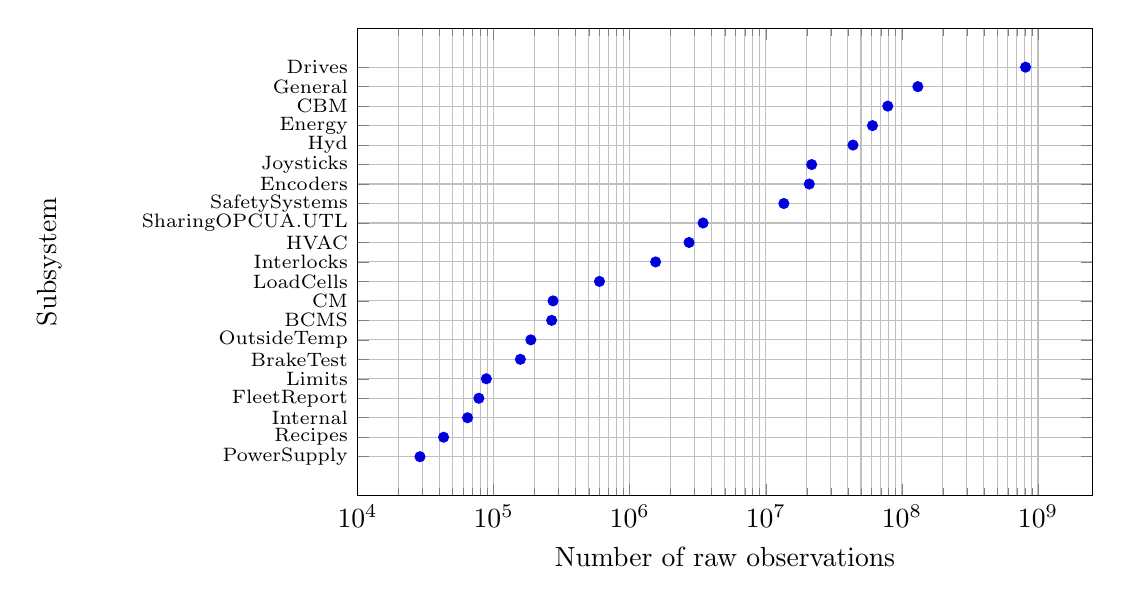
\begin{tikzpicture}
    \begin{axis}[
        width=0.9\linewidth,
        height=0.62\linewidth,
        xmode=log,
        xlabel={Number of raw observations},
        ylabel={Subsystem},
        y dir=reverse,
        ytick={1,2,3,4,5,6,7,8,9,10,11,12,13,14,15,16,17,18,19,20,21},
        yticklabels={
{Drives},
{General},
{CBM},
{Energy},
{Hyd},
{Joysticks},
{Encoders},
{SafetySystems},
{SharingOPCUA.UTL},
{HVAC},
{Interlocks},
{LoadCells},
{CM},
{BCMS},
{OutsideTemp},
{BrakeTest},
{Limits},
{FleetReport},
{Internal},
{Recipes},
{PowerSupply}
        },
        yticklabel style={font=\scriptsize, text width=0.28\linewidth, align=right},
        grid=both,
        xmin=10000
    ]
        \addplot+[only marks, mark=*, mark size=1.8pt] coordinates {
(809883172,1)
(130908115,2)
(78698273,3)
(60742482,4)
(43673540,5)
(21716740,6)
(20842339,7)
(13561207,8)
(3457524,9)
(2727855,10)
(1548304,11)
(598856,12)
(273023,13)
(266715,14)
(187495,15)
(157128,16)
(88324,17)
(77823,18)
(64260,19)
(42840,20)
(28732,21)
        };
    \end{axis}
    \end{tikzpicture}
    \caption{Observation volume by tag subsystem.}
    \label{fig:subsystem-observation-volume}
\end{figure}
